%% RCA-SMOTE: Mitigating Rare Minority Subgroup Starvation in Cluster-Based Oversampling
%% Elsevier elsarticle class, default single-column preprint layout (a4paper, 10pt), numbered references (elsarticle-num).

\documentclass[preprint,nopreprintline]{elsarticle}

\usepackage{graphicx}
\usepackage{url}
\usepackage{amsmath,amssymb,amsfonts}
\usepackage{amsthm}
\usepackage{textcomp}
\usepackage{booktabs}
\usepackage{algorithm}
\usepackage{algorithmicx}
\usepackage{algpseudocode}
\usepackage{needspace}
\usepackage{adjustbox}
\usepackage[hidelinks]{hyperref}

\setlength{\emergencystretch}{1.5em}

\theoremstyle{plain}
\newtheorem{proposition}{Proposition}
\theoremstyle{definition}
\newtheorem{definition}{Definition}

\newcommand{\wba}{\mathrm{wBA}}
\newcommand{\rg}{R_{G}}
\newcommand{\tabfont}{\fontsize{8}{9.4}\selectfont}
\providecommand{\botrule}{\bottomrule}

%% float placement: allow figures and tables to share pages with text
\renewcommand{\topfraction}{0.92}
\renewcommand{\bottomfraction}{0.8}
\renewcommand{\textfraction}{0.06}
\renewcommand{\floatpagefraction}{0.85}
\setcounter{topnumber}{3}
\setcounter{bottomnumber}{2}
\setcounter{totalnumber}{4}

\begin{document}

\begin{frontmatter}

\title{RCA-SMOTE: Mitigating Rare Minority Subgroup Starvation in Cluster-Based Oversampling}


\author{Divya Yadav}
\ead{divyayadav4344@gmail.com}
\author{Mayankkumar Rathva}
\ead{mayankrathva281@gmail.com}
\author{Pratipalsinh Jadeja}
\ead{Pratipaljadeja8@gmail.com}
\author{Sankhadeep Chatterjee}
\ead{sdc.svnit@gmail.com}

\begin{abstract}
Cluster-based oversamplers are designed to respect the internal structure of the minority class, yet the step that organises this class into clusters can leave its rarest parts without any synthetic samples. We call this failure subgroup starvation and study it in the released implementation of AW-SMOTE, a recent density- and boundary-weighted oversampler. We identify two mechanisms: its DBSCAN configuration excludes roughly the sparsest 35\% of minority points from generation, and clusters without majority neighbours receive a zero quota. We propose RCA-SMOTE, which excludes a sparse point only when all five of its nearest training neighbours are majority points, allocates the synthetic budget in proportion to the square root of cluster size, and generates samples by SMOTE-style interpolation. On 19 datasets with known minority subgroups, evaluated with 5$\times$2-fold cross-validation and four classifiers, RCA-SMOTE reduced the share of training folds in which the smallest subgroup received no synthetic sample from 34.2\% to 0.5\%. Relative to AW-SMOTE, it raised weighted balanced accuracy from 0.822 to 0.853 and smallest-subgroup recall from 0.556 to 0.674, at the cost of slightly lower specificity; in dataset-level tests of an earlier run of the benchmark, both gains were significant (Holm-adjusted $p<0.001$ and $p=0.004$). Its mean values were also slightly higher than those of standard SMOTE (0.849 and 0.641), although these small differences do not by themselves establish significant superiority. Ablation identified the rescue rule as the most robust component, and adding the rescue and quota corrections to KMeans-SMOTE and DBSMOTE raised their weighted balanced accuracy by 0.035 and 0.023 while lowering precision. The results call for subgroup-aware evaluation of cluster-based oversampling; they do not show that any method is universally superior.
\end{abstract}

\begin{keyword}
Imbalanced classification \sep Oversampling \sep Intra-class imbalance \sep Small disjuncts \sep SMOTE \sep DBSCAN \sep Subgroup starvation
\end{keyword}

\end{frontmatter}

%% =====================================================================================
\section{Introduction}\label{sec:intro}

This section explains why the internal structure of the minority class matters, identifies the gap that motivates the study and states our contributions.

\subsection{Background and motivation}\label{sec:background}

In imbalanced classification, the class of interest has far fewer training examples than the others, and learners that minimise an aggregate loss drift towards the majority class \cite{japkowicz2002class,he2009learning}. The class ratio is only part of the difficulty. Class overlap, borderline and noisy examples, and the fragmentation of a class into small regions can matter as much as the ratio itself \cite{prati2004class,napierala2016types}. This paper is about the last factor. A minority class often consists of subconcepts of very different sizes, such as disease subtypes or fault modes that share a label but occupy different regions of the feature space. This intra-class imbalance creates small disjuncts that classifiers learn poorly \cite{holte1989concept,japkowicz2001concept,jo2004class}. The resulting errors are easy to miss, because recall, F1, G-mean and ROC-AUC are dominated by the largest subconcept \cite{bellinger2024performance}.

Oversampling is the most common remedy. Cluster-based oversamplers first partition the minority class and then share the synthetic budget among the clusters, precisely to respect its internal structure \cite{jo2004class,douzas2018kmeans,bunkhumpornpat2012dbsmote}. The same machinery can, however, defeat its own purpose: a sparse subgroup that is labelled as noise, or that is assigned no budget, receives no synthetic support at all.

\subsection{Research gap and objectives}\label{sec:gap}

Earlier work noted that denoising may remove valid rare examples \cite{napierala2016types}, and the authors of AW-SMOTE \cite{yan2026awsmote} call the complete removal of DBSCAN noise a strong assumption. What has not been reported is how often cluster-based oversamplers actually leave a known minority subgroup without synthetic samples, which mechanisms are responsible, and whether correcting them changes subgroup-level performance. Aggregate benchmarks cannot answer these questions, because they do not record subgroup membership. Our objectives are (i) to formalise this failure and identify its mechanisms, (ii) to measure it on datasets with known subgroups, (iii) to design and evaluate a correction, RCA-SMOTE (rare-cluster-aware SMOTE), without tuning it on the evaluation data, and (iv) to test whether the corrections transfer to other cluster-based oversamplers, taking the released implementation of AW-SMOTE \cite{yan2026awsmote} as the base case.

\subsection{Main contributions}\label{sec:contrib}

\begin{enumerate}
\item A formal definition of subgroup starvation, and an analysis of two properties of the released AW-SMOTE configuration that can each starve a rare subgroup (Section~\ref{sec:problem}).
\item RCA-SMOTE, which combines sparse-point rescue, size-based allocation and SMOTE-style generation, described at the level of the frozen implementation, including its edge cases (Section~\ref{sec:method}).
\item A 51-dataset benchmark in which RCA-SMOTE reduces observed starvation, improves on AW-SMOTE with dataset-level statistical support, and reaches mean performance close to, and on several metrics slightly above, that of standard SMOTE (Section~\ref{sec:results}).
\item Ablation, sensitivity and transfer experiments that locate the gain mainly in the rescue rule and show that the corrections reduce starvation in KMeans-SMOTE and DBSMOTE, at a cost in precision (Section~\ref{sec:mechanism}).
\item A re-analysis of all inferential claims with datasets as independent blocks, and a cautious reconstruction of the original AW-SMOTE benchmark (Section~\ref{sec:discussion}).
\end{enumerate}

%% =====================================================================================
\section{Related work}\label{sec:related}

We review general oversampling methods, cluster-based oversampling and work on rare subconcepts, and then summarise the properties of AW-SMOTE that motivate this study.

\subsection{Traditional oversampling techniques}\label{sec:rw-over}

SMOTE \cite{chawla2002smote} places a synthetic point $\mathbf{x}+\lambda(\mathbf{x}'-\mathbf{x})$, $\lambda\sim U[0,1]$, between a minority example $\mathbf{x}$ and one of its $k$ nearest minority neighbours $\mathbf{x}'$. It remains a strong reference across benchmarks \cite{fernandez2018smote,kovacs2019empirical}. ADASYN \cite{he2008adasyn} gives more synthetic points to examples with many majority neighbours, Borderline-SMOTE \cite{han2005borderline} and SVM-SMOTE \cite{nguyen2011borderline} restrict generation to the class boundary, and hybrid methods add cleaning with Tomek links or edited nearest neighbours \cite{batista2004study,tomek1976two,wilson1972asymptotic}. All of these methods treat the minority class as one population, and the boundary-oriented variants deliberately move synthetic points away from regions far from the majority class.

\subsection{Cluster-based and boundary-aware oversampling}\label{sec:rw-cluster}

Cluster-based oversampling (CBO) \cite{jo2004class} clusters each class and enlarges every cluster to the size of the largest one, as a direct response to small disjuncts. KMeans-SMOTE \cite{douzas2018kmeans} keeps $k$-means clusters with a sufficient minority share and favours sparse clusters, and DBSMOTE \cite{bunkhumpornpat2012dbsmote} applies DBSCAN \cite{ester1996density} to the minority class. MWMOTE \cite{barua2014mwmote}, CBSO \cite{barua2011cbso}, A-SUWO \cite{nekooeimehr2016asuwo}, SOMO \cite{douzas2017somo}, CURE-SMOTE \cite{ma2017cure} and Cluster-SMOTE \cite{cieslak2006combating} combine clustering with boundary or density weighting. AW-SMOTE \cite{yan2026awsmote} belongs to this family. It clusters the minority class with DBSCAN, discards DBSCAN noise, allocates the budget by a boundary weight per cluster, and interpolates within clusters using a sigmoid fusion of boundary and density weights. Its authors report strong F1, G-mean and AUC values on 16 KEEL datasets.

\subsection{Intra-class imbalance and rare subgroups}\label{sec:rw-intra}

The link between rare subconcepts and classification error goes back to the study of small disjuncts \cite{holte1989concept}. Japkowicz \cite{japkowicz2001concept} and Jo and Japkowicz \cite{jo2004class} argued that within-class imbalance explains much of the damage usually attributed to between-class imbalance. Napierala and Stefanowski \cite{napierala2016types} labelled minority examples as safe, borderline, rare or outlier according to the composition of their neighbourhoods; their distinction between rare examples and outliers is the basis of our rescue rule. Recent surveys still list within-class structure as an open problem \cite{krawczyk2016learning}. Bellinger et al. \cite{bellinger2024performance} built benchmarks with known minority subconcepts and showed that standard measures are biased towards the largest one; we follow their construction principle.

\subsection{Limitations of AW-SMOTE}\label{sec:rw-aw}

In the released AW-SMOTE implementation, a percentile radius labels an almost fixed fraction of the minority class as noise, and a boundary-weighted quota gives nothing to clusters away from the majority class (Section~\ref{sec:mechanisms}); the code also departs from the published specification in several details (Section~\ref{sec:aw-repro}). None of this is visible in aggregate F1, G-mean or AUC, which is how starvation can go unnoticed in a benchmark.

%% =====================================================================================
\section{Problem formulation and subgroup starvation analysis}\label{sec:problem}

We define subgroup starvation, show how the released AW-SMOTE configuration produces it and derive the requirements that guide the design of RCA-SMOTE.

\subsection{Formal problem definition}\label{sec:formal}

Let $\mathcal{D}=\{(\mathbf{x}_i,y_i)\}_{i=1}^{n}$, $\mathbf{x}_i\in\mathbb{R}^d$, $y_i\in\{0,1\}$, with minority set $\mathcal{P}=\{\mathbf{x}_i:y_i=1\}$ and majority set $\mathcal{Q}$, $m=|\mathcal{P}|<M=|\mathcal{Q}|$ and $\mathrm{IR}=M/m$.

\begin{definition}[Minority subgroups]\label{def:subgroups}
The minority class is partitioned into disjoint subgroups $\mathcal{P}=\bigcup_{g=1}^{G}\mathcal{S}_g$, $G\ge2$, ordered so that $|\mathcal{S}_1|\ge\dots\ge|\mathcal{S}_G|$. Subgroup labels $s(\mathbf{x})$ are known to the evaluator but never given to the oversampler or the classifier.
\end{definition}

An oversampler returns $\mathcal{D}\cup\mathcal{Z}$ with $|\mathcal{Z}|=N=M-m$ synthetic minority points. A cluster-based oversampler partitions a retained subset $\mathcal{P}^{*}\subseteq\mathcal{P}$ into clusters $C_1,\dots,C_K$ and assigns integer quotas $n_j\ge0$ with $\sum_jn_j=N$. Points of $\mathcal{P}\setminus\mathcal{P}^{*}$ are excluded from generation but stay in the training set. Because synthetic points carry no subgroup label, each one is attributed to the subgroup of its nearest original minority point:
\begin{equation}\label{eq:attribution}
a(\mathbf{z})=s\bigl(\arg\min_{\mathbf{x}\in\mathcal{P}}\lVert\mathbf{z}-\mathbf{x}\rVert_2\bigr),\qquad N_g=|\{\mathbf{z}\in\mathcal{Z}:a(\mathbf{z})=g\}|.
\end{equation}

\begin{definition}[Subgroup starvation]\label{def:starvation}
Subgroup $g$ is starved in a training fold if $N_g=0$. The starvation rate of a method is the percentage of training folds in which the smallest subgroup $\mathcal{S}_G$ is starved.
\end{definition}

Eq.~\eqref{eq:attribution} is a proxy, because it does not identify the seed from which each synthetic point was generated. We therefore also report a coverage proxy: the percentage of original minority points that are the nearest original point of at least one synthetic point. On a test set, the recall of subgroup $g$ and the specificity are
\begin{equation}\label{eq:subrecall}
R_g=\frac{|\{\mathbf{x}\in\mathcal{T}_g:\hat y(\mathbf{x})=1\}|}{|\mathcal{T}_g|},\qquad \mathrm{Spec}=\frac{|\{\mathbf{x}\in\mathcal{T}_0:\hat y(\mathbf{x})=0\}|}{|\mathcal{T}_0|},
\end{equation}
where $\mathcal{T}_g$ and $\mathcal{T}_0$ are the test points of subgroup $g$ and of the majority class; $\rg$ is the smallest-subgroup recall.

\subsection{Mechanisms of subgroup starvation}\label{sec:mechanisms}

\begin{figure}[!htb]
\centering
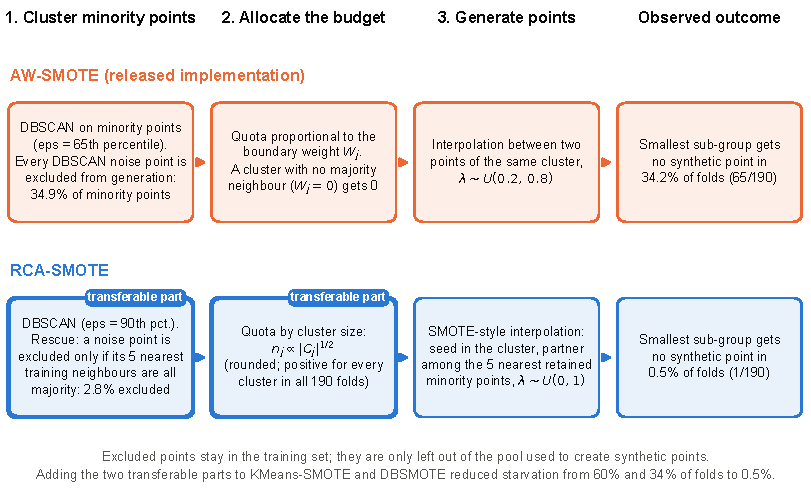
\includegraphics[width=0.96\textwidth]{../figures/fig1_methodology.pdf}
\caption{Where AW-SMOTE loses rare subgroups and how RCA-SMOTE changes each stage. The released AW-SMOTE implementation excludes every DBSCAN noise point from generation and gives a zero quota to clusters without majority neighbours. RCA-SMOTE uses a coarser radius, excludes a noise point only when its five nearest training neighbours are all majority points, allocates the budget in proportion to $|C_j|^{1/2}$ and interpolates towards one of the five nearest retained minority points. The two marked components are transferred to other methods in Section~\ref{sec:transfer}. Percentages are means over the 190 training folds of the 19 Group A-main datasets.}
\label{fig:method}
\end{figure}

Fig.~\ref{fig:method} summarises the two mechanisms. Let $d_1(\mathbf{x})$ be the distance from $\mathbf{x}\in\mathcal{P}$ to its nearest other minority point. AW-SMOTE sets the DBSCAN radius to $\varepsilon=\mathrm{Perc}_{65}\{d_1(\mathbf{x})\}$ with $\textit{MinPts}=2$, where the count includes the point itself.

\begin{proposition}\label{prop:noise}
With $\textit{MinPts}=2$ and closed $\varepsilon$-neighbourhoods, the DBSCAN noise set of $\mathcal{P}$ is $\{\mathbf{x}:d_1(\mathbf{x})>\varepsilon\}$. If $\varepsilon$ is the $q$-th percentile of the values $d_1$, the fraction of noise points is approximately $1-q/100$, up to ties and percentile interpolation, whatever the data.
\end{proposition}

\begin{proof}
A point is core if its $\varepsilon$-neighbourhood contains another point, that is, if $d_1(\mathbf{x})\le\varepsilon$. A non-core point joins a cluster only if it lies within $\varepsilon$ of a core point, which also implies $d_1(\mathbf{x})\le\varepsilon$. Hence $\mathbf{x}$ is noise if and only if $d_1(\mathbf{x})>\varepsilon$.
\end{proof}

With $q=65$, about 35\% of the minority class is excluded by construction (34.9\% measured). The excluded points are those with the largest nearest-neighbour distances, which is exactly where a sparse subgroup lies. For the allocation, the implementation counts the majority points $b(\mathbf{x})$ among the five nearest training neighbours of $\mathbf{x}$ (the query included), sets $W_j=\max_{\mathbf{x}\in C_j}b(\mathbf{x})$ and $n_j=\mathrm{round}(NW_j/\sum_lW_l)$, and adds the rounding residual to the largest quota.

\begin{proposition}\label{prop:zero}
If $W_j=0$ and $\sum_lW_l>0$, then $n_j=0$ before the residual step, and the residual step changes only the cluster with the largest rounded quota.
\end{proposition}

A compact rare subgroup in a safe region \cite{napierala2016types} therefore receives nothing whenever another cluster touches the majority class. The released code produced 3.3 zero-quota clusters per fold on average, and its small radius fragments subgroups: on the development data it found 15.2 clusters for three to four true subgroups. Both propositions describe the configuration; whether a subgroup is actually starved is measured empirically in Section~\ref{sec:starvation}.

\subsection{Motivation for subgroup-aware resampling}\label{sec:motivation}

In the two-dimensional example of Fig.~\ref{fig:example}, all eight points of a sparse subgroup (S3) are DBSCAN noise. AW-SMOTE therefore generates nothing near them, whereas RCA-SMOTE attributes 121 of its 524 synthetic points to S3. Fig.~\ref{fig:starvation} shows that the problem is confined neither to toy data nor to one method. Two requirements follow: sparse points should not be discarded merely for being sparse, and no cluster should receive zero samples merely because it is far from the majority class. RCA-SMOTE is designed to meet both requirements while keeping generation close to SMOTE.

\begin{figure}[!htb]
\centering
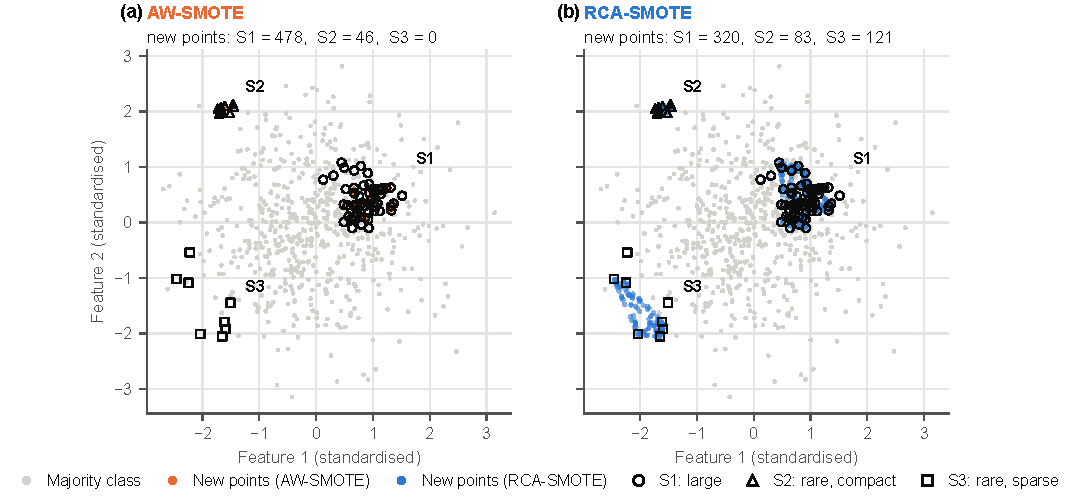
\includegraphics[width=0.92\textwidth]{../figures/fig2_synthetic_example.pdf}
\caption{Two-dimensional illustration with a large subgroup (S1), a compact rare subgroup (S2) and a sparse rare subgroup (S3); hollow markers are original minority points and dots are synthetic points. (a) AW-SMOTE (released implementation) generates nothing near S3. (b) RCA-SMOTE generates points for all three subgroups. Counts use the attribution of Eq.~\eqref{eq:attribution} (seed 0). The example is descriptive.}
\label{fig:example}
\end{figure}

\begin{figure}[!htb]
\centering
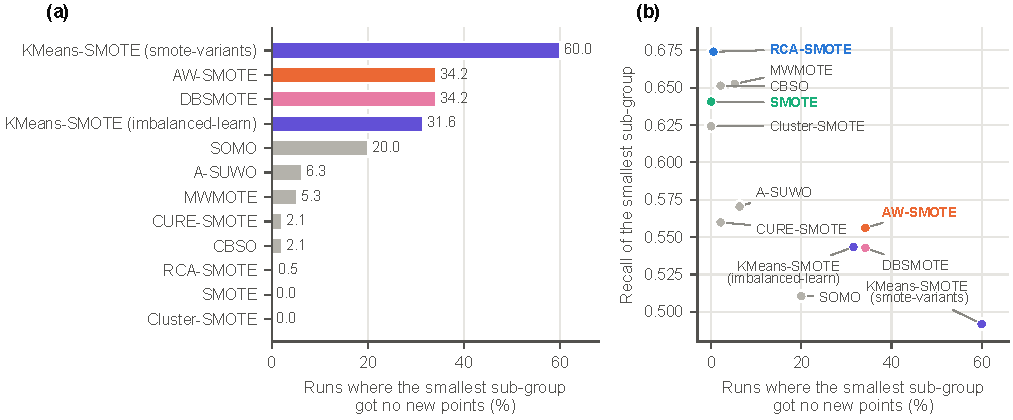
\includegraphics[width=0.94\textwidth]{../figures/fig3_starvation.pdf}
\caption{Starvation across oversamplers on Group A-main. (a) Percentage of the 190 training folds in which the smallest subgroup received no synthetic point; eight cluster-based methods use smote-variants defaults, and KMeans-SMOTE also appears in its imbalanced-learn version with the fallback policy of Section~\ref{sec:methods-compared}. (b) Starvation rate against mean smallest-subgroup recall for the 12 methods. Starvation rates and the recalls of the other methods are from the earlier run (Table~\ref{tab:starvation}); RCA-SMOTE is plotted at its updated $\rg$ (0.674, Table~\ref{tab:groupA}). The methods share data and design elements, so the panel is descriptive and implies no causal relation.}
\label{fig:starvation}
\end{figure}

%% =====================================================================================
\section{Proposed method: RCA-SMOTE}\label{sec:method}

This section describes the frozen RCA-SMOTE stage by stage and ends with the complete algorithm and its computational cost.

\subsection{Overview of the proposed framework}\label{sec:overview}

RCA-SMOTE keeps the three stages of AW-SMOTE, namely clustering, allocation and generation, and changes each of them (Fig.~\ref{fig:method}). The design was chosen among nine variants on five development datasets by a rule fixed in advance (highest mean weighted balanced accuracy) and then frozen. The method handles binary problems, treats the less frequent label as the minority class and expects standardised features.

\subsection{Minority clustering and sparse-point rescue}\label{sec:clustering}

RCA-SMOTE sets $\varepsilon=\mathrm{Perc}_{90}\{d_1(\mathbf{x}):\mathbf{x}\in\mathcal{P}\}$ and runs DBSCAN with $\textit{MinPts}=2$, so about 10\% of minority points are noise before rescue (Proposition~\ref{prop:noise}). If duplicates make $\varepsilon=0$, the smallest positive $d_1$ is used (or $10^{-6}$); the same guard is applied to AW-SMOTE. If all points are noise, they form one cluster. A noise point $\mathbf{x}$ is excluded from generation only if
\begin{equation}\label{eq:rescue}
y(\mathbf{x}')=0\quad\text{for all }\mathbf{x}'\in\mathcal{K}_5(\mathbf{x}),
\end{equation}
where $\mathcal{K}_5(\mathbf{x})$ are its five nearest neighbours in the training set, excluding itself. This rule follows the distinction between rare examples, which have some support from their own class, and outliers, which are surrounded by the other class \cite{napierala2016types}. Excluded points remain in the training data. A rescued point joins the cluster of its nearest clustered minority point if that distance is at most $\tau=\mathrm{Perc}_{95}\{d_1\}$. The remaining rescued points $\mathcal{U}$ form one cluster if $|\mathcal{U}|=1$; otherwise they are grouped by single linkage with threshold
\begin{equation}\label{eq:taur}
\tau_r=\max\bigl(\tau,\;2\,\mathrm{median}_{\mathbf{u}\in\mathcal{U}}\,d_1^{\,\mathcal{U}}(\mathbf{u})\bigr),
\end{equation}
where $d_1^{\,\mathcal{U}}$ is the nearest-neighbour distance within $\mathcal{U}$. In this way a widely spaced subgroup can still form one micro-cluster. The final clusters $C_1,\dots,C_K$ cover the retained pool $\mathcal{P}^{*}$.

\subsection{Cluster-size-based quota allocation}\label{sec:quota}

The budget $N=M-m$ is allocated by cluster size only:
\begin{equation}\label{eq:quota}
q_j=\frac{|C_j|^{1-\beta}}{\sum_{l=1}^{K}|C_l|^{1-\beta}},\qquad n_j=\mathrm{round}(Nq_j),\qquad \beta=0.5,
\end{equation}
with NumPy rounding and the residual $N-\sum_jn_j$ added to the largest rounded quota (an inherited weight for AW-SMOTE's boundary term is set to zero). With $\beta=0$, each original point receives the same expected number of synthetic points, as in SMOTE; with $\beta=1$, each cluster receives the same number, as in CBO \cite{jo2004class}. The value $\beta=0.5$ lies between these extremes and gives points of small clusters proportionally more.

\begin{proposition}\label{prop:ratio}
Ignoring rounding, if $|C_a|>|C_b|>0$ and $0<\beta\le1$, then $(|C_a|+Nq_a)/(|C_b|+Nq_b)<|C_a|/|C_b|$.
\end{proposition}

\begin{proof}
With $a=|C_a|$, $b=|C_b|$ and $c=N/\sum_l|C_l|^{1-\beta}$, the claim $(a+ca^{1-\beta})/(b+cb^{1-\beta})<a/b$ reduces to $b^{\beta}<a^{\beta}$.
\end{proof}

The proposition concerns discovered clusters, not true subgroups, and does not imply that every subgroup receives synthetic points. Eq.~\eqref{eq:quota} also has no lower bound: a cluster with $Nq_j<0.5$ can receive zero, and because the whole residual goes to one cluster, degenerate inputs can even produce a negative quota (a constructed case with ten duplicate pairs and class counts $(26,20)$ yields $(-3,1,\dots,1)$). This did not occur in the evaluation, where every cluster in the 190 main training folds received a positive quota (minimum 5) and the total equalled $N$. A general minimum of one point per cluster is impossible when $N<K$.

\subsection{Synthetic sample generation}\label{sec:generation}

For each cluster with $n_j>0$, the seed indices $0,\dots,n_j-1$ are taken modulo $|C_j|$ and shuffled, so each member is used $\lfloor n_j/|C_j|\rfloor$ or $\lceil n_j/|C_j|\rceil$ times (the first $n_j$ members when $n_j<|C_j|$). For seed $\mathbf{x}$, a partner $\mathbf{p}$ is drawn uniformly from its $\min(5,|\mathcal{P}^{*}|-1)$ nearest points in $\mathcal{P}^{*}$, possibly in another cluster, and
\begin{equation}\label{eq:interp}
\mathbf{z}=\mathbf{x}+\lambda(\mathbf{p}-\mathbf{x}),\qquad\lambda\sim U[0,1).
\end{equation}
The quota decides where synthetic points originate, while the choice of partner follows SMOTE. Singleton clusters can therefore generate points, at the price that some points fall between subgroups, as they do in SMOTE.

\subsection{Algorithm summary and computational complexity}\label{sec:algorithm}

\begin{algorithm}[!htb]
\caption{RCA-SMOTE (frozen configuration)}\label{alg:rca}
\begin{algorithmic}[1]
\small
\Require training set $\mathcal{D}$ with standardised features; $\textit{MinPts}=2$, $k=5$, $\beta=0.5$, seed
\State $N\gets|\mathcal{Q}|-|\mathcal{P}|$; \textbf{if} $N\le0$ \textbf{return} $\mathcal{D}$
\State $\varepsilon\gets\mathrm{Perc}_{90}(d_1)$ with zero-radius guard; $\tau\gets\mathrm{Perc}_{95}(d_1)$; DBSCAN$(\varepsilon,\textit{MinPts})$ on $\mathcal{P}$; $\mathcal{N}\gets$ noise
\ForAll{$\mathbf{x}\in\mathcal{N}$}
  \If{all $k$ nearest training neighbours of $\mathbf{x}$ are majority} exclude $\mathbf{x}$ from generation
  \ElsIf{nearest clustered minority point within $\tau$} join its cluster
  \Else{} add $\mathbf{x}$ to $\mathcal{U}$
  \EndIf
\EndFor
\State group $\mathcal{U}$ by single linkage with threshold $\tau_r$ (Eq.~\ref{eq:taur}); add groups as clusters; $\mathcal{P}^{*}\gets\bigcup_jC_j$
\State $n_j\gets\mathrm{round}(N|C_j|^{1-\beta}/\sum_l|C_l|^{1-\beta})$; add $N-\sum_jn_j$ to the largest $n_j$
\ForAll{$C_j$ with $n_j>0$, seeds $\mathbf{x}\in$ shuffle$((0..n_j-1)\bmod|C_j|)$}
  \State draw $\mathbf{p}$ among the $\min(k,|\mathcal{P}^{*}|-1)$ nearest points of $\mathbf{x}$ in $\mathcal{P}^{*}$; $\lambda\sim U[0,1)$
  \State $\mathcal{Z}\gets\mathcal{Z}\cup\{\mathbf{x}+\lambda(\mathbf{p}-\mathbf{x})\}$
\EndFor
\State \Return $\mathcal{D}\cup\mathcal{Z}$, all points of $\mathcal{Z}$ labelled minority
\end{algorithmic}
\end{algorithm}

Algorithm~\ref{alg:rca} summarises the procedure. With $n=m+M$ and brute-force neighbour search, the minority distances and DBSCAN cost $O(m^2d)$, the rescue test $O(|\mathcal{N}|nd)$, single linkage $O(|\mathcal{U}|^2d)$ time and $O(|\mathcal{U}|^2)$ memory, the partner search $O(m^2d)$ and the interpolation $O(Nd)$. The implementation also computes boundary counts that receive zero weight, an avoidable $O(mnd)$ step. The total is $O((mn+m^2)d+Nd)$ time and $O(nd+|\mathcal{U}|^2)$ memory. The mean resampling time per training fold over all 51 datasets was 0.093\,s for RCA-SMOTE, 0.298\,s for AW-SMOTE and 0.009\,s for SMOTE (descriptive measurements from parallel runs).

%% =====================================================================================
\section{Experimental setup}\label{sec:setup}

This section describes the data, the compared methods, the metrics and the statistical procedures; Table~\ref{tab:datasets} summarises the protocol.

\subsection{Dataset description and partitioning}\label{sec:data}

The study uses 51 datasets (Table~\ref{tab:datasets}). Group A comprises 24 datasets with known minority subgroups, built from multi-class data following Bellinger et al. \cite{bellinger2024performance}. Classes with fewer than ten examples are dropped, the larger half of the remaining classes forms the majority class (subsampled to at most 2000 examples), and up to four further classes become minority subgroups; the first is capped at $\max(\lfloor M/10\rfloor,40)$ examples and each later one is about half the size of the previous one (minimum ten). The five development datasets (A-dev) were used only for design selection. The ten A-held datasets had been used once before to test the frozen method, and SMOTE and AW-SMOTE results on them had been seen before the development split. The nine A-new datasets (five from PMLB \cite{olson2017pmlb}, four from OpenML-CC18 \cite{vanschoren2014openml}) were admitted by a rule written in advance and had not been used before. A-held and A-new together form \emph{Group A-main} (19 datasets), the basis of all primary claims. Group B contains 27 binary benchmarks with unknown subgroup structure from KEEL \cite{alcala2011keel} and imbalanced-learn \cite{lemaitre2017imbalanced}, including the 13 datasets of the AW-SMOTE study. Six of them share raw data with Group A and are excluded in the B-no-overlap analysis (21 datasets).

\begin{table}[!htb]
\caption{Dataset groups and protocol. Ranges over the datasets of each subset; $n$: examples; $d$: features after encoding; IR: imbalance ratio; $G$: minority subgroups.}\label{tab:datasets}
\centering\tabfont
\setlength{\tabcolsep}{3pt}
\begin{adjustbox}{max width=\textwidth}
\begin{tabular}{@{}llrccccl@{}}
\toprule
Subset & Source & Sets & $n$ & $d$ & IR & $G$ & Role \\
\midrule
A-dev & PMLB & 5 & 290--2375 & 7--40 & 3.14--8.20 & 3--4 & design only \\
A-held & PMLB & 10 & 202--2375 & 5--64 & 2.88--13.26 & 2--4 & A-main (used once) \\
A-new & PMLB, OpenML & 9 & 224--2350 & 13--216 & 3.00--6.74 & 2--4 & A-main (new) \\
B-KEEL (AW) & KEEL & 13 & 215--1066 & 3--41 & 1.86--68.10 & -- & AW-SMOTE study \\
B-KEEL (extra) & KEEL & 8 & 150--4174 & 4--13 & 1.82--129.44 & -- & benchmark \\
B-imblearn & imblearn & 6 & 531--2536 & 49--294 & 10.80--33.74 & -- & benchmark \\
\midrule
\multicolumn{8}{@{}p{0.96\textwidth}@{}}{\textit{Protocol:} 5$\times$2-fold cross-validation stratified by subgroup (A) or class (B); scaling and resampling fitted on training folds only; 16 resampling configurations and 4 ensembles; SVM (RBF, $C$=1), $k$NN ($k$=5), decision tree, random forest (100 trees); seeds equal to the fold index; statistical unit: dataset (mean of 10 folds, then of 4 classifiers).} \\
\botrule
\end{tabular}
\end{adjustbox}
\end{table}

\subsection{Competing methods and classifiers}\label{sec:methods-compared}

Sixteen resampling configurations were compared: no resampling; random oversampling (ROS), SMOTE \cite{chawla2002smote}, ADASYN \cite{he2008adasyn}, Borderline-SMOTE \cite{han2005borderline}, SVM-SMOTE \cite{nguyen2011borderline}, KMeans-SMOTE \cite{douzas2018kmeans}, AW-SMOTE \cite{yan2026awsmote} and RCA-SMOTE; random undersampling (RUS), NearMiss-1, ClusterCentroids, Tomek links \cite{tomek1976two} and edited nearest neighbours (ENN) \cite{wilson1972asymptotic}; and the hybrids SMOTEENN and SMOTETomek \cite{batista2004study}. Library methods are taken from imbalanced-learn 0.14.2 \cite{lemaitre2017imbalanced} with default settings and neighbour counts of five. Balanced random forest, balanced bagging, EasyEnsemble \cite{liu2009exploratory} and RUSBoost \cite{seiffert2010rusboost} were compared separately with random forest plus resampling. AW-SMOTE is the authors' released code at a pinned commit, unchanged except for the shared zero-radius guard; its mask misalignment and $[0.2,0.8]$ interpolation range were retained. With default settings, KMeans-SMOTE found no usable cluster in 245 of 510 folds; it was then rerun with relaxed settings (173 folds) or replaced by SMOTE (72 folds, all in Group B), so its row describes this fallback policy. ADASYN (five folds) and SVM-SMOTE (two folds) occasionally failed, in which case the original data were used; RUSBoost failed in four folds after ten seed retries, and RCA-SMOTE and AW-SMOTE never failed. All classifiers used scikit-learn \cite{pedregosa2011scikit} defaults and the default decision rule; the random forest follows \cite{breiman2001random}.

\subsection{Evaluation metrics}\label{sec:metrics}

With TP, FP, TN and FN counted for the minority class: $\mathrm{Acc}=(TP+TN)/(TP+TN+FP+FN)$, $\mathrm{Prec}=TP/(TP+FP)$, $\mathrm{Rec}=TP/(TP+FN)$, $\mathrm{Spec}=TN/(TN+FP)$, $F_1=2TP/(2TP+FP+FN)$, $\mathrm{BA}=(\mathrm{Rec}+\mathrm{Spec})/2$, $\text{G-mean}=\sqrt{\mathrm{Rec}\cdot\mathrm{Spec}}$ and
\begin{equation}\label{eq:mcc}
\mathrm{MCC}=\frac{TP\cdot TN-FP\cdot FN}{\sqrt{(TP+FP)(TP+FN)(TN+FP)(TN+FN)}},
\end{equation}
with precision and MCC set to zero for vanishing denominators \cite{chicco2020advantages}. ROC-AUC uses the SVM decision function or predicted probabilities, and PR-AUC is average precision \cite{saito2015precision}. The two central metrics are subgroup-aware. Weighted balanced accuracy gives half of the weight to the majority class and divides the other half equally among the subgroups,
\begin{equation}\label{eq:wba}
\wba=\tfrac{1}{2}\bigl(\mathrm{Spec}+\tfrac{1}{G}\textstyle\sum_{g=1}^{G}R_g\bigr),
\end{equation}
so that, unlike BA, it is not dominated by the largest subgroup, in the spirit of the instance-weighted measures of \cite{bellinger2024performance}. The smallest-subgroup recall $\rg$ refers to the subgroup that is smallest by construction, not to the one with the lowest observed recall. The primary metrics, fixed in advance, are $\wba$ and $\rg$ for Group A and G-mean and MCC for Group B.

\subsection{Cross-validation and statistical testing}\label{sec:stats}

Each dataset was evaluated with five repetitions of two-fold cross-validation \cite{dietterich1998approximate}, with scaling and resampling fitted on the training half only \cite{kaufman2012leakage,santos2018cross}. Fold values were averaged per dataset, classifier and method, and the four classifier means were then averaged with equal weight. Because the four classifiers share datasets and folds, treating the 76 dataset--classifier pairs of Group A-main as independent, as earlier project analyses did, overstates the sample size. All inferences here therefore use datasets as blocks ($n=19$ for A-main, 9 for A-new, 27 and 21 for Group B). Pairwise comparisons use the two-sided Wilcoxon signed-rank test \cite{wilcoxon1945individual} with Holm correction \cite{holm1979simple} within declared families: RCA-SMOTE against the 15 other configurations per metric and subset, six ablation configurations per metric, and six metrics per transferred method. The Friedman test \cite{friedman1937use} with the Nemenyi critical difference $\mathrm{CD}=q_{0.05}(k,\infty)\sqrt{k(k+1)/(6n)}/\sqrt{2}$, equal to 5.29 ranks for $k=16$, $n=19$ \cite{demsar2006statistical}, assesses all configurations jointly. The all-pairs Nemenyi procedure is conservative for any single pair and can disagree with a targeted Holm-corrected test \cite{demsar2006statistical}, so both are reported. Non-significance is never read as equivalence; no equivalence test was performed.

%% =====================================================================================
\section{Experimental results and comparative analysis}\label{sec:results}

We report results on the subgroup-aware benchmark (Group A-main) and the standard benchmarks (Group B), then analyse subgroup recall and summarise the statistical tests.

\subsection{Performance on subgroup-aware benchmarks}\label{sec:resA}

\begin{table}[!htb]
\caption{Group A-main (19 datasets): dataset-level means of the 16 configurations. RCA-SMOTE: updated measurements; other methods: earlier run (Section~\ref{sec:resA}). Rows are ordered by the historical mean rank on $\wba$ from the earlier run, which was not recomputed for the updated RCA-SMOTE means. Bold: best displayed value per column. Tests (earlier run) are in Table~\ref{tab:stats}.}\label{tab:groupA}
\centering\tabfont
\setlength{\tabcolsep}{4.2pt}
\begin{adjustbox}{max width=\textwidth}
\begin{tabular}{@{}lcccccccc@{}}
\toprule
Method & $\wba$ & $\rg$ & G-mean & F1 & MCC & Prec. & Spec. & Hist.\ rank ($\wba$) \\
\midrule
SVM-SMOTE & 0.849 & 0.631 & 0.858 & 0.751 & 0.709 & 0.724 & 0.938 & \textbf{4.11} \\
SMOTETomek & 0.850 & 0.640 & \textbf{0.862} & 0.753 & 0.710 & 0.725 & 0.932 & 4.18 \\
SMOTE & 0.849 & 0.641 & 0.861 & 0.752 & 0.709 & 0.724 & 0.932 & 4.71 \\
\textbf{RCA-SMOTE} & \textbf{0.853} & 0.674 & 0.861 & \textbf{0.759} & \textbf{0.719} & 0.744 & 0.936 & 5.37 \\
ADASYN & 0.849 & 0.668 & 0.858 & 0.733 & 0.687 & 0.689 & 0.918 & 5.47 \\
SMOTEENN & 0.841 & 0.681 & 0.860 & 0.708 & 0.656 & 0.635 & 0.870 & 5.74 \\
ROS & 0.843 & 0.612 & 0.852 & 0.754 & 0.715 & 0.749 & 0.943 & 6.84 \\
Borderline-SMOTE & 0.844 & 0.625 & 0.854 & 0.741 & 0.696 & 0.712 & 0.930 & 6.89 \\
RUS & 0.833 & 0.653 & 0.854 & 0.684 & 0.629 & 0.597 & 0.854 & 8.53 \\
ENN & 0.827 & 0.557 & 0.841 & 0.736 & 0.688 & 0.720 & 0.930 & 9.11 \\
KMeans-SMOTE$^{a}$ & 0.823 & 0.543 & 0.832 & 0.747 & 0.708 & 0.776 & 0.953 & 10.42 \\
AW-SMOTE & 0.822 & 0.556 & 0.830 & 0.733 & 0.691 & 0.743 & 0.949 & 11.05 \\
ClusterCentroids & 0.820 & 0.709 & 0.831 & 0.663 & 0.602 & 0.582 & 0.811 & 11.74 \\
TomekLinks & 0.806 & 0.495 & 0.787 & 0.725 & 0.700 & 0.813 & 0.976 & 12.71 \\
No resampling & 0.802 & 0.485 & 0.780 & 0.720 & 0.698 & \textbf{0.819} & \textbf{0.978} & 13.71 \\
NearMiss-1 & 0.752 & \textbf{0.719} & 0.749 & 0.531 & 0.441 & 0.421 & 0.676 & 15.42 \\
\botrule
\end{tabular}
\end{adjustbox}
\par\smallskip\raggedright\footnotesize $^{a}$ imbalanced-learn with the fallback policy of Section~\ref{sec:methods-compared}.
\end{table}

Table~\ref{tab:groupA} reports Group A-main. The RCA-SMOTE rows of Tables~\ref{tab:groupA} and~\ref{tab:groupB} are updated aggregate measurements. All other rows come from the earlier run of the benchmark, which an independent rerun (190 dataset folds, 12,160 resampler--classifier fits) reproduced exactly at fold level. In that earlier run, RCA-SMOTE reached $\wba$ 0.847 and $\rg$ 0.631 on Group A-main. The dataset-level tests, mean ranks and per-dataset counts reported below, and the analyses of Section~\ref{sec:mechanism}, were computed on the earlier run and were not recomputed for the updated means.

Against AW-SMOTE, RCA-SMOTE raised $\wba$ from 0.822 to 0.853 and $\rg$ from 0.556 to 0.674 (Fig.~\ref{fig:datasetwise}). In the earlier run, it was higher on 19 and 18 of the 19 datasets, respectively (Holm-adjusted $p=5.7\times10^{-5}$ and $0.0040$). F1, MCC and G-mean also rose, whereas specificity fell from 0.949 to 0.936 (adjusted $p=0.037$ in the earlier run). RCA-SMOTE thus detects more minority cases at the price of more false positives. The single negative case in the earlier run, satimage, gained 0.3 points in $\wba$ but lost 10.9 points in $\rg$, so a better subgroup balance on average does not guarantee a better result for every subgroup.

\begin{figure}[!htb]
\centering
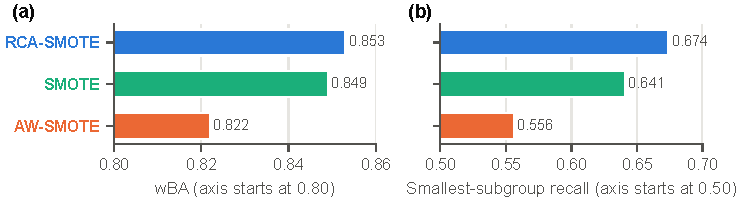
\includegraphics[width=0.80\textwidth]{../figures/fig4_dataset_comparison.pdf}
\caption{Method-level means across the 19 Group A-main datasets for RCA-SMOTE, SMOTE and AW-SMOTE: (a) $\wba$, (b) smallest-subgroup recall $\rg$ (values of Table~\ref{tab:groupA}; each dataset averaged over four classifiers and ten folds; RCA-SMOTE: updated measurements). The bars are aggregate means, not dataset-level differences. The axes do not start at zero.}
\label{fig:datasetwise}
\end{figure}

Against SMOTE, the reported means favour RCA-SMOTE slightly on $\wba$ (0.853 vs 0.849), $\rg$ (0.674 vs 0.641), F1 (0.759 vs 0.752) and MCC (0.719 vs 0.709). These differences are small, and higher means alone do not establish that RCA-SMOTE is significantly better than SMOTE. SMOTEENN, ClusterCentroids and NearMiss-1 reach a higher $\rg$, but they lose so much precision and specificity that their $\wba$ and MCC are not higher. In the earlier run, RCA-SMOTE exceeded AW-SMOTE on every one of the nine previously unused A-new datasets ($\wba$ 0.806 vs 0.778; $\rg$ 0.649 vs 0.562). With nine pairs, however, the Holm-adjusted $p$ cannot fall below 0.059, so this unanimous direction is not significant at 0.05, and SMOTE had a higher $\wba$ than RCA-SMOTE on eight of the nine. On the development datasets, RCA-SMOTE reached $\wba$ 0.822, SMOTE 0.823 and AW-SMOTE 0.806.

\subsection{Performance on standard imbalanced benchmarks}\label{sec:resB}

\begin{table}[!htb]
\caption{Group B (27 binary benchmarks): dataset-level means, ordered by G-mean. RCA-SMOTE: updated measurements; other methods: earlier run. Bold: best displayed value per column, ties included.}\label{tab:groupB}
\centering\tabfont
\begin{adjustbox}{max width=\textwidth}
\begin{tabular}{@{}lccccccc@{}}
\toprule
Method & G-mean & MCC & F1 & ROC-AUC & PR-AUC & Recall & Spec. \\
\midrule
RUS & \textbf{0.763} & 0.391 & 0.428 & 0.814 & 0.433 & \textbf{0.777} & 0.767 \\
SMOTEENN & 0.744 & 0.442 & 0.483 & \textbf{0.823} & 0.446 & 0.690 & 0.855 \\
ClusterCentroids & 0.727 & 0.377 & 0.418 & 0.803 & 0.434 & \textbf{0.777} & 0.734 \\
\textbf{RCA-SMOTE} & 0.693 & \textbf{0.457} & \textbf{0.502} & 0.817 & 0.474 & 0.588 & 0.914 \\
SMOTETomek & 0.681 & 0.442 & 0.486 & 0.815 & 0.464 & 0.576 & 0.912 \\
SMOTE & 0.680 & 0.440 & 0.485 & 0.815 & 0.464 & 0.574 & 0.912 \\
ADASYN & 0.675 & 0.427 & 0.473 & 0.812 & 0.452 & 0.576 & 0.903 \\
SVM-SMOTE & 0.663 & 0.452 & 0.496 & 0.811 & 0.472 & 0.551 & 0.927 \\
Borderline-SMOTE & 0.661 & 0.442 & 0.487 & 0.808 & 0.463 & 0.553 & 0.918 \\
KMeans-SMOTE$^{a}$ & 0.647 & 0.442 & 0.479 & 0.811 & 0.470 & 0.516 & 0.938 \\
ROS & 0.641 & 0.437 & 0.479 & 0.799 & 0.462 & 0.523 & 0.931 \\
NearMiss-1 & 0.629 & 0.276 & 0.353 & 0.703 & 0.364 & 0.730 & 0.602 \\
AW-SMOTE & 0.624 & 0.420 & 0.465 & 0.799 & 0.452 & 0.502 & 0.927 \\
ENN & 0.586 & 0.428 & 0.467 & 0.810 & 0.473 & 0.508 & 0.916 \\
TomekLinks & 0.519 & 0.406 & 0.430 & 0.800 & \textbf{0.480} & 0.404 & 0.962 \\
No resampling & 0.504 & 0.399 & 0.418 & 0.797 & \textbf{0.480} & 0.383 & \textbf{0.969} \\
\botrule
\end{tabular}
\end{adjustbox}
\par\smallskip\raggedright\footnotesize $^{a}$ includes 72 folds in which plain SMOTE replaced KMeans-SMOTE.
\end{table}

On Group B (Table~\ref{tab:groupB}), which includes AW-SMOTE's own benchmark datasets, RCA-SMOTE improved on AW-SMOTE in G-mean (0.693 vs 0.624) and MCC (0.457 vs 0.420). In the dataset-level tests of the earlier run, both advantages were significant (G-mean higher on 26 of 27 datasets, adjusted $p=4.5\times10^{-7}$; MCC adjusted $p=0.013$), also without the overlapping datasets. Its reported mean G-mean, F1 and MCC (0.693, 0.502 and 0.457) were also slightly higher than those of SMOTE (0.680, 0.485 and 0.440) and SMOTETomek (0.681, 0.486 and 0.442). As on Group A, these mean differences do not by themselves establish significant superiority; in the earlier run, RCA-SMOTE's G-mean was slightly below that of both methods (Table~\ref{tab:stats}). RUS, SMOTEENN and ClusterCentroids led on G-mean through high recall, at a clear cost in MCC, precision and specificity.

\subsection{Minority subgroup recall analysis}\label{sec:subgroup}

Fig.~\ref{fig:subgroup} places the updated mean smallest-subgroup recall of RCA-SMOTE (0.674) among all 16 configurations. It is the fourth highest, above AW-SMOTE (0.556), SMOTE (0.641) and ADASYN (0.668), and below only NearMiss-1, ClusterCentroids and SMOTEENN, which obtain their higher $\rg$ at a large cost in precision and specificity (Table~\ref{tab:groupA}). Recalls by subgroup position exist only for the earlier run, where recall fell from the largest to the smallest subgroup for every method. The mean recalls of subgroups 1--4 were 0.834, 0.803, 0.694 and 0.625 for RCA-SMOTE, 0.787, 0.739, 0.628 and 0.517 for AW-SMOTE, 0.842, 0.809, 0.701 and 0.642 for SMOTE, and 0.718, 0.665, 0.564 and 0.453 without resampling (subgroups 3 and 4 exist on only 16 and 10 datasets). RCA-SMOTE lay above AW-SMOTE at every position and close to SMOTE, but the gap of about 0.2 between the largest and the smallest subgroup remained for both. In the same earlier run, balanced random forest exceeded random forest with RCA-SMOTE on $\wba$ (0.859 vs 0.848, adjusted $p=0.010$) and EasyEnsemble exceeded it on $\rg$ (0.695 vs 0.566, adjusted $p=0.003$), whereas random forest with RCA-SMOTE had a higher MCC than all four ensembles.

\subsection{Statistical comparison of competing methods}\label{sec:statcomp}

In the earlier run, the Friedman test rejected equal performance of the 16 configurations on Group A-main ($p<10^{-19}$ for both primary metrics). On $\wba$, RCA-SMOTE's mean rank of 5.37 was close to those of SMOTE, SMOTETomek and SVM-SMOTE (Table~\ref{tab:groupA}) and 5.68 ranks ahead of AW-SMOTE, more than the critical difference of 5.29. On $\rg$ the gap was 5.11 ranks, so the all-pairs procedure did not separate the two methods, whereas the targeted Holm-corrected test did (adjusted $p=0.0040$), in line with the different error control of the two procedures (Section~\ref{sec:stats}). Table~\ref{tab:stats} collects every inferential comparison. Beyond the primary metrics, SMOTE had significantly higher minority recall ($-0.008$ for RCA-SMOTE, adjusted $p=0.002$) and RCA-SMOTE significantly higher specificity ($+0.004$, adjusted $p=0.020$), so the two methods sat at slightly different points of the same recall--specificity trade-off. Fig.~\ref{fig:rankings} shows the updated mean $\wba$ of all 16 configurations as aggregate means, not as mean ranks or a critical-difference analysis. The slightly higher mean $\wba$, F1 and MCC of RCA-SMOTE in Table~\ref{tab:groupA} are therefore not by themselves evidence of a difference in overall quality.

%% =====================================================================================
\section{Mechanism analysis, ablation and transferability}\label{sec:mechanism}

This section examines why the results above arise: we measure starvation directly, revert the components of RCA-SMOTE, vary its parameters and add its corrections to other oversamplers. All analyses here come from the earlier run.

\subsection{Quantifying minority subgroup starvation}\label{sec:starvation}

\begin{table}[!htb]
\caption{Starvation and coverage on the 190 Group A-main training folds. Starved: folds in which the smallest subgroup received no synthetic point (Eq.~\ref{eq:attribution}). Share: synthetic points attributed to the smallest subgroup (its share of real minority points is 14.7\%). Coverage: original minority points that are the nearest original point of a synthetic point. Excl.: minority points excluded from generation, where measurable. Maj.: synthetic points with at least three majority points among their five nearest original training points.}\label{tab:starvation}
\centering\tabfont
\setlength{\tabcolsep}{3pt}
\begin{adjustbox}{max width=\textwidth}
\begin{tabular}{@{}llcccccc@{}}
\toprule
Method & Lib. & Starved & (\%) & Share (\%) & Coverage (\%) & Excl. (\%) & Maj. (\%) \\
\midrule
SMOTE & IL & 0 & (0.0) & 14.0 & 95.6 & -- & 19.6 \\
ROS & IL & 0 & (0.0) & 14.8 & 97.0 & -- & 24.9 \\
ADASYN & IL & 9 & (4.7) & 20.1 & 71.6 & -- & 36.1 \\
Borderline-SMOTE & IL & 18 & (9.5) & 20.3 & 57.9 & -- & 28.9 \\
SVM-SMOTE & IL & 1 & (0.5) & 16.8 & 73.9 & -- & 17.1 \\
KMeans-SMOTE$^{a}$ & IL & 60 & (31.6) & 10.7 & 60.7 & -- & 13.1 \\
AW-SMOTE & RC & 65 & (34.2) & 16.6 & 43.6 & 34.9 & 31.3 \\
\textbf{RCA-SMOTE} & -- & 1 & (0.5) & 17.3 & 93.3 & 2.8 & 19.5 \\
\midrule
KMeans-SMOTE & SV & 114 & (60.0) & 21.5 & 29.8 & 48.8$^{b}$ & 6.3 \\
DBSMOTE & SV & 65 & (34.2) & 14.5 & 41.9 & 56.6 & 15.6 \\
SOMO & SV & 38 & (20.0) & 20.3 & 33.3 & -- & 21.2 \\
A-SUWO & SV & 12 & (6.3) & 29.6 & 37.4 & 10.0$^{c}$ & 46.6 \\
MWMOTE & SV & 10 & (5.3) & 14.7 & 86.4 & -- & 25.2 \\
CBSO & SV & 4 & (2.1) & 21.6 & 74.0 & -- & 45.8 \\
CURE-SMOTE & SV & 4 & (2.1) & 21.8 & 65.4 & -- & 24.1 \\
Cluster-SMOTE & SV & 0 & (0.0) & 18.7 & 91.9 & -- & 18.9 \\
\botrule
\end{tabular}
\end{adjustbox}
\par\smallskip\raggedright\footnotesize Lib.: IL imbalanced-learn, SV smote-variants, RC released authors' code. $^{a}$ with fallback policy; $^{b}$ points in clusters filtered out by the method; $^{c}$ points removed from the data as noise.
\end{table}

Table~\ref{tab:starvation} quantifies starvation. The released AW-SMOTE starved the smallest subgroup in 65 of 190 folds and excluded about a third of the minority points, and its synthetic points were nearest to fewer than half of them. RCA-SMOTE starved it in a single fold and reached a coverage close to that of SMOTE. Starvation is not specific to AW-SMOTE: with smote-variants defaults \cite{kovacs2019smotevariants}, KMeans-SMOTE, DBSMOTE and SOMO starved the smallest subgroup in 60\%, 34\% and 20\% of folds. The causes match Section~\ref{sec:mechanisms}. KMeans-SMOTE filters out clusters with few minority points and distributes the budget by random draws, and DBSMOTE excludes DBSCAN noise. The imbalanced-learn version of KMeans-SMOTE starved less, mainly because of its permissive fallback settings; with their own defaults, both libraries starved in about half of 113 comparable folds. These findings concern default implementations, not the underlying ideas.

The single remaining RCA-SMOTE case is instructive. In fold 2 of vowel, all five training points of the smallest subgroup were DBSCAN noise with five majority nearest neighbours each, so the rescue rule classified them as outliers. RCA-SMOTE reduces starvation; it does not guarantee that every true subgroup is represented. Nor is a large share for the smallest subgroup desirable in itself: A-SUWO and CBSO have high shares but place over 45\% of their points in majority-dominated regions, against 19.5\% for RCA-SMOTE.

\subsection{Component ablation study}\label{sec:ablation}

\begin{table}[!htb]
\caption{Leave-one-component-out ablation on Group A-main ($n=19$). Each row reverts one component to its AW-SMOTE counterpart. $\Delta$: difference from full RCA-SMOTE in percentage points; Low.: datasets on which the reverted version is lower; $p_\mathrm{H}$: Holm-adjusted over six configurations per metric (bold: $<0.05$); Starv., Excl.: percentages of starved folds and excluded minority points. All rows, including the full method, are from the earlier run (Section~\ref{sec:resA}); the full-method row therefore differs from the updated RCA-SMOTE means of Table~\ref{tab:groupA}.}\label{tab:ablation}
\centering\tabfont
\setlength{\tabcolsep}{2.2pt}
\begin{adjustbox}{max width=\textwidth}
\begin{tabular}{@{}lcccccccccc@{}}
\toprule
 & \multicolumn{4}{c}{$\wba$} & \multicolumn{3}{c}{$\rg$} & MCC & & \\
\cmidrule(lr){2-5}\cmidrule(lr){6-8}
Configuration & Mean & $\Delta$ & Low. & $p_\mathrm{H}$ & Mean & $\Delta$ & $p_\mathrm{H}$ & Mean & Starv. & Excl. \\
\midrule
\textbf{RCA-SMOTE (full)} & 0.8472 & -- & -- & -- & 0.6311 & -- & -- & 0.7104 & 0.5 & 2.8 \\
No rescue & 0.8410 & $-0.62$ & 18 & \textbf{0.0001} & 0.6124 & $-1.87$ & 0.080 & 0.7034 & 2.6 & 10.5 \\
AW quota & 0.8415 & $-0.57$ & 14 & 0.092 & 0.6136 & $-1.74$ & 0.197 & 0.7017 & 7.4 & 2.8 \\
AW clustering ($\varepsilon_{65}$) & 0.8458 & $-0.13$ & 13 & 0.434 & 0.6251 & $-0.60$ & 0.340 & 0.7094 & 0.5 & 6.4 \\
AW generation & 0.8442 & $-0.29$ & 13 & 0.434 & 0.6209 & $-1.02$ & 0.212 & 0.7041 & 0.5 & 2.8 \\
AW gen.\ (aligned) & 0.8449 & $-0.22$ & 10 & 0.515 & 0.6293 & $-0.18$ & 0.931 & 0.7008 & 0.5 & 2.8 \\
All four (= AW-SMOTE) & 0.8224 & $-2.48$ & 19 & \textbf{$<$0.0001} & 0.5561 & $-7.50$ & \textbf{0.002} & 0.6906 & 34.2 & 34.9 \\
\botrule
\end{tabular}
\end{adjustbox}
\par\smallskip\raggedright\footnotesize Exact adjusted $p$-values for $\wba$: no rescue $1.3\times10^{-4}$; all four $2.3\times10^{-5}$. AW generation: the released AW-SMOTE generation stage; mask aligned: the same stage with its majority mask corrected.
\end{table}

Each of RCA-SMOTE's four components was reverted to its AW-SMOTE counterpart, one at a time and all together (Table~\ref{tab:ablation}, Fig.~\ref{fig:ablation}); reverting all four reproduces AW-SMOTE exactly, including its starvation. Removing the rescue rule is the only single-component change whose effect survives correction: it lowered $\wba$ on 18 of 19 datasets and almost quadrupled the share of excluded minority points. Reverting to the boundary-weighted quota cost a similar mean amount and caused the largest single rise in starvation, but its effect varied more across datasets and is not significant. The clustering and generation components had smaller, non-significant effects on the primary metrics, although the quota and the mask-aligned generation significantly lowered MCC (adjusted $p=0.011$ and $0.042$). Reverting all four components cost more than the sum of the four single effects shown in Fig.~\ref{fig:ablation} ($-2.48$ against $-1.62$ points on $\wba$), so the components compensate for each other; without rescue, for example, the size quota still prevents most starvation (2.6\% instead of 34.2\%). Because each reversion also changes the clustering seen by later stages and the random-number sequence, the rows show conditional effects, not independent causal contributions.

\begin{figure}[!htb]
\centering
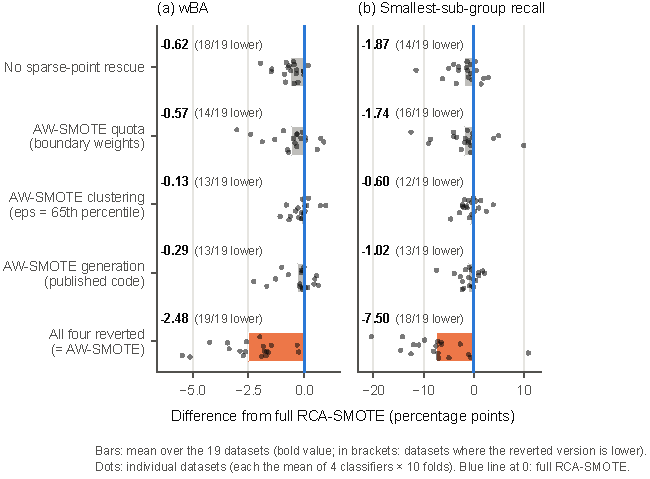
\includegraphics[width=0.74\textwidth]{../figures/fig5_ablation.pdf}
\caption{Ablation on Group A-main: change in (a) $\wba$ and (b) $\rg$, in percentage points, when one component or all four are reverted to AW-SMOTE. Bars: means over datasets; dots: datasets (four classifiers, ten folds); brackets: datasets on which the reverted version is lower. After Holm correction only the $\wba$ loss without rescue and both losses with all four reverted are significant. Label ``published code'': the released implementation. Earlier run (Table~\ref{tab:ablation}).}
\label{fig:ablation}
\end{figure}

\subsection{Parameter sensitivity analysis}\label{sec:sensitivity}

We varied one parameter at a time: the radius percentile (50--99), the quota exponent $\beta$ (0--1) and the neighbour counts for partners and for the rescue test (3--10). Mean $\wba$ stayed between 0.841 and 0.849 (default 0.847), against 0.822 for AW-SMOTE and 0.849 for SMOTE. The largest change came from $\beta=1$, which gives equal budgets per cluster as in CBO. It lowered $\wba$ by 0.007 and $\rg$ by 0.026 and raised starvation to 2.1\%, because it spreads the budget thinly over many small clusters. A few settings were marginally better than the default (rescue with ten neighbours, $+0.0015$), but the frozen default was not changed. These one-at-a-time results do not establish joint robustness.

\subsection{Transferability to other cluster-based oversamplers}\label{sec:transfer}

\begin{table}[!htb]
\caption{Adding the rescue rule and the size-based quota to KMeans-SMOTE and DBSMOTE (smote-variants defaults) on Group A-main: dataset-level means. $\Delta$: change from the original method to the version with both components, with Holm-adjusted $p$-values over six metrics in parentheses. Transfer rows: earlier run.}\label{tab:transfer}
\centering\tabfont
\setlength{\tabcolsep}{2.4pt}
\begin{adjustbox}{max width=\textwidth}
\begin{tabular}{@{}lcccccccc@{}}
\toprule
Method & Starved & Excl. & $\wba$ & $\rg$ & Prec. & Spec. & F1 & MCC \\
\midrule
KMeans-SMOTE & 60.0 & 48.8 & 0.806 & 0.492 & 0.798 & 0.972 & 0.722 & 0.694 \\
\quad + rescue & 35.3 & 10.0 & 0.813 & 0.518 & 0.787 & 0.968 & 0.724 & 0.694 \\
\quad + quota & 51.6 & 48.8 & 0.810 & 0.496 & 0.789 & 0.970 & 0.725 & 0.696 \\
\quad + both & 0.5 & 10.0 & 0.842 & 0.606 & 0.740 & 0.944 & 0.753 & 0.710 \\
\quad $\Delta$ (both) & & & $+0.035$ & $+0.114$ & $-0.057$ & $-0.028$ & $+0.031$ & $+0.016$ \\
 & & & \scriptsize($<$0.001) & \scriptsize($<$0.001) & \scriptsize($<$0.001) & \scriptsize($<$0.001) & \scriptsize(0.072) & \scriptsize(0.113) \\
\midrule
DBSMOTE & 34.2 & 56.6 & 0.815 & 0.543 & 0.781 & 0.961 & 0.731 & 0.696 \\
\quad + rescue & 0.5 & 8.6 & 0.837 & 0.588 & 0.757 & 0.950 & 0.753 & 0.714 \\
\quad + quota & 34.2 & 56.6 & 0.816 & 0.543 & 0.780 & 0.960 & 0.730 & 0.696 \\
\quad + both & 0.5 & 8.6 & 0.838 & 0.591 & 0.753 & 0.949 & 0.751 & 0.712 \\
\quad $\Delta$ (both) & & & $+0.023$ & $+0.048$ & $-0.028$ & $-0.012$ & $+0.021$ & $+0.016$ \\
 & & & \scriptsize($<$0.001) & \scriptsize(0.011) & \scriptsize(0.011) & \scriptsize(0.006) & \scriptsize(0.008) & \scriptsize(0.014) \\
\midrule
\textbf{RCA-SMOTE} (ref.)$^{a}$ & 0.5 & 2.8 & 0.853 & 0.674 & 0.744 & 0.936 & 0.759 & 0.719 \\
SMOTE (ref.)$^{a}$ & 0.0 & -- & 0.849 & 0.641 & 0.724 & 0.932 & 0.752 & 0.709 \\
\botrule
\end{tabular}
\end{adjustbox}
\par\smallskip\raggedright\footnotesize $^{a}$ $\wba$ to MCC: means of Table~\ref{tab:groupA} (RCA-SMOTE: updated measurements); starvation and exclusion: Table~\ref{tab:starvation}.
\end{table}

We added the rescue rule, the size quota or both to the smote-variants implementations of KMeans-SMOTE and DBSMOTE, keeping each method's own clustering and generation; with both disabled, the code reproduces the library output. For DBSMOTE, rescue applies the rules of Section~\ref{sec:clustering} to DBSCAN noise. For KMeans-SMOTE, it keeps the minority points of discarded clusters unless they satisfy Eq.~\eqref{eq:rescue}, but it also recomputes cluster membership and merges singleton groups, which is a broader intervention than a single switch. The transferred quota is proportional to $|C_j|^{1/2}$, with a minimum of one point per cluster.

\begin{figure}[!htb]
\centering
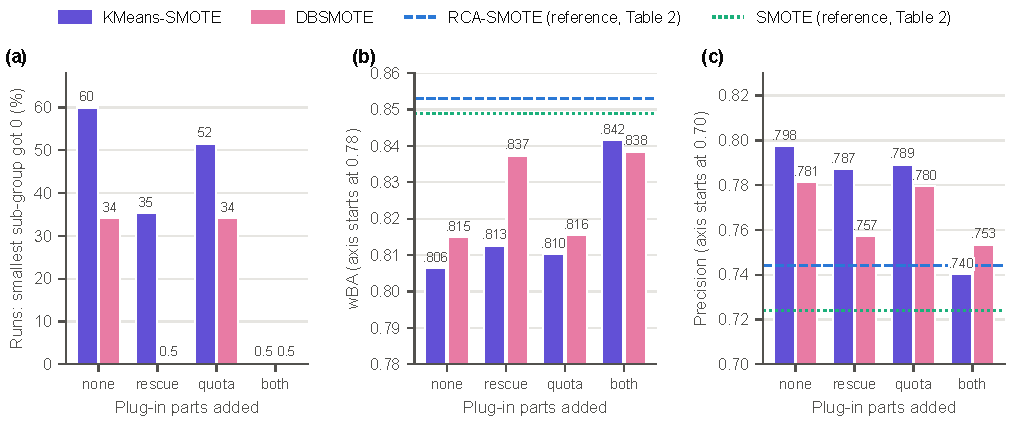
\includegraphics[width=0.94\textwidth]{../figures/fig6_transferability.pdf}
\caption{Transfer of the corrections to KMeans-SMOTE and DBSMOTE (Group A-main): (a) starvation rate, (b) $\wba$, (c) precision, for the original methods and with rescue, quota or both (earlier run; values of Table~\ref{tab:transfer}). Dashed and dotted lines: means of RCA-SMOTE (updated measurements: $\wba$ 0.853, precision 0.744) and SMOTE (0.849, 0.724) from Table~\ref{tab:groupA}. The axes of (b) and (c) do not start at zero.}
\label{fig:transfer}
\end{figure}

With both components (Table~\ref{tab:transfer}, Fig.~\ref{fig:transfer}), starvation fell to 0.5\% for both methods, and $\wba$ and $\rg$ rose significantly. Which component mattered reflects how each method starves. DBSMOTE loses subgroups through noise exclusion and already allocates by cluster size, so rescue alone removed its starvation. KMeans-SMOTE starves through cluster filtering and random allocation, so only the combination was effective. The gains have a cost: precision and specificity fell significantly for both methods. F1 and MCC still rose, significantly for DBSMOTE but not for KMeans-SMOTE. The corrected methods end slightly below RCA-SMOTE and SMOTE on $\wba$ and clearly below them on $\rg$.

%% =====================================================================================
\section{Discussion and limitations}\label{sec:discussion}

We interpret the findings, discuss the trade-off between minority detection and false positives, examine why our AW-SMOTE results differ from the published ones and list the threats to validity.

\subsection{Interpretation of the main findings}\label{sec:interpretation}

The results form a consistent chain: two properties of the released AW-SMOTE configuration left rare subgroups without synthetic support in a third of the folds; replacing them reduced observed starvation to one fold in 190 and improved mean subgroup-aware performance, on nearly every dataset in the earlier run; the ablation ties most of the gain to the treatment of sparse points; and the same corrections reduce starvation in two other methods. Table~\ref{tab:stats} gives the statistical support for each claim.

\begin{table}[!htb]
\caption{Consolidated dataset-level comparisons. $\Delta$: mean difference (first minus second); W/T/L: datasets on which the first is better, tied or worse; $p$: two-sided Wilcoxon test; $p_\mathrm{H}$: Holm-adjusted within the stated family. ``n.s.'': no significant difference detected at 0.05, not equivalence. All entries were computed on the dataset-level results of the earlier run (RCA-SMOTE $\wba$ 0.847 and $\rg$ 0.631 on Group A-main) and were not recomputed for the updated means of Tables~\ref{tab:groupA} and~\ref{tab:groupB}.}\label{tab:stats}
\centering\tabfont
\setlength{\tabcolsep}{3pt}
\begin{adjustbox}{max width=\textwidth}
\begin{tabular}{@{}llcrccl@{}}
\toprule
Comparison & Metric & $\Delta$ & W/T/L & $p$ & $p_\mathrm{H}$ & Conclusion \\
\midrule
\multicolumn{7}{@{}l}{\textit{Group A-main, $n=19$; family: RCA-SMOTE vs 15 configurations per metric}} \\
RCA vs AW-SMOTE & $\wba$ & $+0.0248$ & 19/0/0 & $3.8\times10^{-6}$ & $5.7\times10^{-5}$ & RCA higher \\
RCA vs AW-SMOTE & $\rg$ & $+0.0750$ & 18/0/1 & $3.4\times10^{-4}$ & 0.0040 & RCA higher \\
RCA vs AW-SMOTE & MCC & $+0.0199$ & 17/0/2 & $9.5\times10^{-5}$ & 0.0010 & RCA higher \\
RCA vs AW-SMOTE & Spec. & $-0.0132$ & 5/0/14 & 0.012 & 0.037 & RCA lower \\
RCA vs SMOTE & $\wba$ & $-0.0022$ & 5/0/14 & 0.104 & 0.625 & n.s. \\
RCA vs SMOTE & $\rg$ & $-0.0096$ & 7/1/11 & 0.177 & 0.885 & n.s. \\
RCA vs SMOTE & MCC & $+0.0011$ & 9/0/10 & 0.891 & 1.000 & n.s. \\
RCA vs SMOTE & Recall & $-0.0076$ & 3/0/16 & $2.1\times10^{-4}$ & 0.0021 & RCA lower \\
RCA vs SMOTE & Spec. & $+0.0037$ & 15/0/4 & 0.0039 & 0.020 & RCA higher \\
\multicolumn{7}{@{}l}{\textit{Group A-new, $n=9$; same family}} \\
RCA vs AW-SMOTE & $\wba$ & $+0.0275$ & 9/0/0 & 0.0039 & 0.059 & n.s.$^{a}$ \\
RCA vs AW-SMOTE & $\rg$ & $+0.0868$ & 9/0/0 & 0.0039 & 0.059 & n.s.$^{a}$ \\
RCA vs SMOTE & $\wba$ & $-0.0022$ & 1/0/8 & 0.0078 & 0.070 & n.s.$^{b}$ \\
\multicolumn{7}{@{}l}{\textit{Group B, $n=27$ (no overlap: $n=21$); same family}} \\
RCA vs AW-SMOTE & G-mean & $+0.0500$ & 26/0/1 & $3.0\times10^{-8}$ & $4.5\times10^{-7}$ & RCA higher \\
RCA vs AW-SMOTE & MCC & $+0.0214$ & 21/0/6 & 0.0010 & 0.013 & RCA higher \\
RCA vs SMOTE & G-mean & $-0.0059$ & 8/0/19 & 0.028 & 0.140 & n.s. \\
RCA vs SMOTE (B-no-ov.) & G-mean & $-0.0068$ & 6/0/15 & 0.060 & 0.261 & n.s. \\
RCA vs SMOTETomek & G-mean & $-0.0070$ & 7/0/20 & 0.0050 & 0.040 & RCA lower \\
\multicolumn{7}{@{}l}{\textit{Ablation, Group A-main, $n=19$; family: six configurations per metric}} \\
No rescue vs full & $\wba$ & $-0.0062$ & 1/0/18 & $2.7\times10^{-5}$ & $1.3\times10^{-4}$ & lower \\
AW quota vs full & $\wba$ & $-0.0057$ & 5/0/14 & 0.023 & 0.092 & n.s. \\
All four reverted vs full & $\rg$ & $-0.0750$ & 1/0/18 & $3.4\times10^{-4}$ & 0.0020 & lower \\
\multicolumn{7}{@{}l}{\textit{Transfer, Group A-main, $n=19$; family: six metrics per base method}} \\
KMeans-SMOTE + both & $\wba$ & $+0.0352$ & 19/0/0 & $3.8\times10^{-6}$ & $2.3\times10^{-5}$ & higher \\
KMeans-SMOTE + both & Prec. & $-0.0571$ & 1/0/18 & $1.9\times10^{-5}$ & $7.6\times10^{-5}$ & lower \\
DBSMOTE + both & $\wba$ & $+0.0235$ & 18/0/1 & $7.6\times10^{-6}$ & $4.6\times10^{-5}$ & higher \\
DBSMOTE + both & Prec. & $-0.0279$ & 3/0/16 & 0.0039 & 0.011 & lower \\
\botrule
\end{tabular}
\end{adjustbox}
\par\smallskip\raggedright\footnotesize $^{a}$ all nine datasets favour RCA-SMOTE; $^{b}$ eight of nine favour SMOTE. Friedman, Group A-main ($k=16$): $\chi^2_{15}=166.1$ ($\wba$) and 128.0 ($\rg$), $p<10^{-19}$; Nemenyi CD $=5.29$.
\end{table}

Why does RCA-SMOTE improve clearly on AW-SMOTE yet end only slightly above SMOTE in mean performance? AW-SMOTE generates only from points that survive denoising and lie in clusters with positive weight, so its coverage is below half and almost a third of its synthetic points fall in majority-dominated regions. RCA-SMOTE's coverage and majority-region share are almost those of SMOTE (Table~\ref{tab:starvation}). What separates the two methods is the square-root quota, which helps rare subgroups only to the extent that discovered clusters coincide with them, and the occasional exclusion of genuine rare points, as in the vowel fold. On balance, RCA-SMOTE and SMOTE remain close: RCA-SMOTE has slightly higher mean specificity and MCC, and the differences are too small to imply a general advantage. In the earlier run, one dataset, vowel, accounted for about 60\% of the signed $\wba$ difference to SMOTE; we report this as a description, not as a reason to exclude it.

\begin{figure}[!htb]
\centering
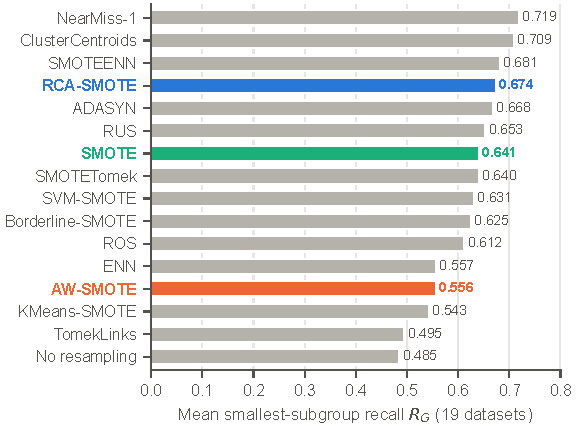
\includegraphics[width=0.62\textwidth]{../figures/fig7_subgroup_recall.pdf}
\caption{Mean smallest-subgroup recall $\rg$ of the 16 configurations over the 19 Group A-main datasets, in descending order (values of Table~\ref{tab:groupA}; RCA-SMOTE: updated measurement). Only the smallest subgroup is shown; recalls by subgroup position are available only for the earlier run (Section~\ref{sec:subgroup}).}
\label{fig:subgroup}
\end{figure}

The subgroup-position recalls of the earlier run (Section~\ref{sec:subgroup}) add a sobering perspective: recall fell with subgroup size for every method, and no configuration in Fig.~\ref{fig:subgroup} reaches a mean $\rg$ above 0.72. Removing starvation is necessary, because a subgroup without synthetic support cannot benefit from oversampling, but it is not sufficient. Interpolation can only densify regions that already contain training points, and on 14 of the 19 datasets the smallest subgroup contributes at most 15 points to a training fold.

\subsection{Performance trade-offs and generalisation}\label{sec:tradeoffs}

Minority detection and false positives trade off throughout. The methods that rank highest on $\rg$, such as NearMiss-1, ClusterCentroids and SMOTEENN, predict the minority class far more often; NearMiss-1 misclassifies about a third of the majority examples. In the earlier run, the ranking of the 16 configurations by $\rg$ was close to the reverse of their rankings by precision and specificity (Kendall $\tau=-0.75$ and $-0.78$) and unrelated or opposite to those by F1 ($-0.28$) and ROC-AUC ($-0.05$). A single aggregate metric would hide this completely. In the dataset-level rankings of the earlier run (Section~\ref{sec:statcomp}), RCA-SMOTE belonged to the leading $\wba$ group with SVM-SMOTE, SMOTETomek, SMOTE, ADASYN and SMOTEENN and occupied a middle position on $\rg$; with 19 datasets and 120 pairs, overlapping groups indicate limited power, not equivalence. On the updated means, RCA-SMOTE has the highest $\wba$ (Fig.~\ref{fig:rankings}), but the eight leading configurations lie within 0.012 of each other.

\begin{figure}[!htb]
\centering
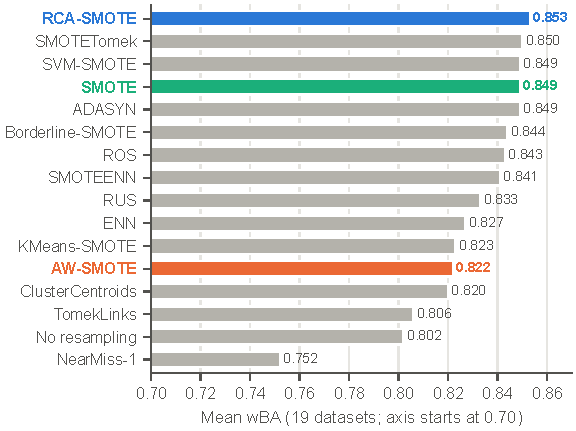
\includegraphics[width=0.62\textwidth]{../figures/fig8_rankings.pdf}
\caption{Mean $\wba$ of the 16 configurations over the 19 Group A-main datasets, in descending order (values of Table~\ref{tab:groupA}; RCA-SMOTE: updated measurement); methods tied at three decimals keep the order of Table~\ref{tab:groupA}. The chart shows aggregate means only; it is not a mean-rank or critical-difference diagram and implies no significance grouping. The axis does not start at zero.}
\label{fig:rankings}
\end{figure}

The corrections address a general mechanism of cluster-based oversampling, yet every corrected method converged towards SMOTE: the corrected KMeans-SMOTE and DBSMOTE stayed below it, and RCA-SMOTE exceeded it only slightly in mean performance. On these data, the value of cluster structure seems to lie mainly in avoiding the harm of exclusion and zero allocation. Once that harm is removed, cluster-aware allocation adds little to SMOTE's neighbourhood interpolation.

\subsection{Reproducibility of the AW-SMOTE baseline}\label{sec:aw-repro}

Our AW-SMOTE scores are much lower than those in the original article \cite{yan2026awsmote}. The evaluated baseline is the released implementation, which differs from the published specification: its generation stage applies the majority mask to a re-ordered matrix, draws the interpolation coefficient from $[0.2,0.8]$ rather than $(0,1)$, uses a different rounding and residual rule, and retains denoised points in the output. Correcting only the mask changed little, so our comparison concerns the released code, not every element of the published specification. We also reconstructed the original benchmark separately from our main 5$\times$2 protocol, with 13 KEEL datasets, five-fold stratified cross-validation, the article's four classifiers and resampling confined to training folds. AW-SMOTE reached a mean F1 of 0.5425, against 0.9309 reported. A deliberately invalid control that scaled and oversampled the full dataset before cross-validation \cite{santos2018cross,kaufman2012leakage} gave 0.9301, with similar agreement for G-mean, AUC and three larger datasets. This is compatible with a difference in the order of resampling and cross-validation, but no experiment runner or fold predictions are available, so how the original experiments were conducted remains unconfirmed. Within the reconstruction, RCA-SMOTE's mean F1 (0.5583) was close to SMOTE's (0.5549), and its G-mean advantage over AW-SMOTE was significant (adjusted $p=0.003$). 

\subsection{Limitations and threats to validity}\label{sec:limitations}

\emph{Subgroup construction.} The Group A subgroups are regrouped original classes with imposed sizes. They may be more separable than natural, overlapping subconcepts, and the results may not transfer to such structure. \emph{Inference.} Nineteen datasets give limited power, the A-new subset cannot reach significance across 15 comparisons, Holm families were defined per metric and subset, and cross-method correlations are observational. All tests, ranks, per-dataset counts and the analyses of Section~\ref{sec:mechanism} come from the earlier run, so the updated mean differences in Tables~\ref{tab:groupA} and~\ref{tab:groupB} are descriptive. \emph{Prior exposure.} The ten A-held datasets had been used once before, and earlier SMOTE and AW-SMOTE results on them had been seen; only A-new was entirely unseen. \emph{Independence.} Seven A-main datasets contain identical labelled feature vectors across folds. Excluding them, the $\wba$ advantage over AW-SMOTE remained significant (adjusted $p=0.007$), but the $\rg$ advantage did not ($p=0.18$). Several Group B datasets are relabellings of common raw data; a source-family analysis with 19 blocks retained the advantages over AW-SMOTE and showed no significant G-mean difference from SMOTE. \emph{Settings.} Methods used library defaults, classifiers were not tuned, and starvation relies on nearest-point attribution. \emph{Method scope.} RCA-SMOTE is limited to binary numerical data. Its rounding has no general non-negativity or minimum guarantee, its seed assignment favours the first cluster members when quotas are small, and self-exclusion in the neighbour search assumes that no duplicate precedes the query point. None of these issues affected the evaluated folds; a revised version would require its own evaluation.

%% =====================================================================================
\section{Conclusion and future work}\label{sec:conclusion}

Cluster-based oversampling can fail the subgroups it is meant to protect. In the released AW-SMOTE implementation, a percentile radius excludes about a third of the minority class from generation regardless of the data, and boundary-weighted allocation gives no budget to clusters away from the majority class. As a result, the smallest subgroup went without synthetic support in a third of the training folds, and default KMeans-SMOTE, DBSMOTE and SOMO showed similar failures. RCA-SMOTE, which replaces these mechanisms with a rescue rule, a square-root size quota and SMOTE-style generation, reduced observed starvation to one fold in 190 and improved mean weighted balanced accuracy and smallest-subgroup recall over AW-SMOTE, with dataset-level statistical support in the earlier run, at a small cost in specificity. Its mean performance was close to, and on several metrics slightly higher than, that of standard SMOTE; these small differences do not establish significant or universal superiority. The rescue rule was the most robust component, and the rescue and quota corrections reduced starvation in KMeans-SMOTE and DBSMOTE while lowering their precision. Because none of these effects was visible in aggregate metrics, cluster-based oversamplers should be evaluated with subgroup-aware measures and explicit starvation statistics.

Beyond the limitations listed in Section~\ref{sec:limitations}, several directions remain open. Future work could develop a bounded apportionment rule that is defined when the budget is smaller than the number of clusters; replace the fixed outlier test with a rule that weighs the risk of discarding a genuine rare subgroup against that of amplifying noise; evaluate the corrections on naturally occurring subconcepts; design generation schemes aimed at the remaining recall gap between large and small subgroups; and compare an equation-faithful AW-SMOTE implementation with the released code under a common protocol.

%% =====================================================================================
\sloppy


%% keep the Declarations block together: it moves to the next page only if it does not fit
\Needspace{16\baselineskip}
\section*{Declarations}

\begin{itemize}
\item \textbf{Funding:} No funding was received to assist with the preparation of this manuscript.
\item \textbf{Conflict of Interest / Competing Interests:} The authors declare that they have no conflict of interest.
\item \textbf{Ethics Approval and Consent to Participate:} Not applicable.
\item \textbf{Consent for Publication:} Not applicable.
\item \textbf{Data Availability:} The datasets referenced in the related works are publicly available, and their URLs are provided in the reference section.
\item \textbf{Materials Availability:} Not applicable.
\item \textbf{Code Availability:} Not applicable.
\item \textbf{Author Contributions:} Divya Yadav contributed to algorithm implementation, experimentation, and validation. Mayankkumar Rathva contributed to conceptualization, methodology development, and manuscript writing. Pratipalsinh Jadeja contributed to data analysis, visualization, and manuscript review. All authors reviewed and approved the final manuscript.
\end{itemize}

\bibliographystyle{elsarticle-num}
\bibliography{references}

\end{document}
